\documentclass[gmd, manuscript]{copernicus} % uncomment to see what the 2 column final paper will look like.

\begin{document}

\section{The emulator}

We treat the output of the simulator $y$ as an uncertain function $f()$ of the simulator inputs $x$, so that $y = f(x)$. We wish to produce a predictive distribution for $y$ at any model input, conditional on the points already run, or the design $(Y, X)$. Throughout the study, we use a kriging function, similar to a Gaussian process regression emulator, as coded in the package DiceKriging \citep{roustant2012dicekriging} in the statistical programming environment R \citep{Rcore2016}, for prediction of climate simulator output at untried inputs.
The kriging model or Gaussian Process regression is specified hierarchically with a separate mean and covariance function. For prediction purposes, \emph{a priori} assume that the trend is a simple linear function of the inputs, and adjust with a Gaussian process. 

%\begin{equation}
$$
f(x) = h(x)^T \beta + Z(x)
$$
%\end{equation}

Where $h(x)^T \beta$ is the mean function, and the residual process $Z$ is a zero mean stationary Gaussian process. The covariance kernel $c$ of $Z$ 

$$
Cov(Z, Z') = \sigma^2 c(x,x')
$$
can be specified in a number of different ways: we use the default diceKriging option of a Matern $v=5/2$ function so that

$$
c(x,x') = (1 + \frac{\sqrt{5} | x - x'|}{\theta} + \frac{5 | x - x'|^2}{3 \theta^2})exp(- \frac{\sqrt{5} |x-x'|}{\theta})
$$

where $\theta$ describes the \emph{characteristic length scales} - a measure of how quickly information about the function is lost moving away from a design point, in any dimension. This and other hyperparameters are estimated via maximum likelihood estimation from the design $(Y, X)$, meaning that the approach is not fully Bayesian (such an approach would find posterior distributions for the hyperparameters rather than point estimates). We use Universal Kriging, with no `nugget' term, meaning that the uncertainty on model outputs shrinks to zero at the design points. 

Full details of the Universal kriging process used can be found in \citep{roustant2012dicekriging}, section 2.1, details of the kernel can be found in section 2.3, and examples of the trend and hyperparameter estimation  in section 3 the same publication. 


\section{Further emulator verification}

Bias correction using the augmented emulator relies on good predictions uing the emulator in the regions of temperature/precipitation space corresponding to observations of the real world. A concern is that there are few ensemble members near the observed values for the Amazon and Central African forests, and that the emulator is forced to extrapolate to estimate forest fraction at these locations. Gaussian process emulators can sometimes perform poorly in extrapolation. Further, it is a concern that the lack of ensemble members near the observations means it is difficult to est the accuracy of the emulator at these important locations.

In an ideal world, we would generate ensemble members at or near the observations in question, as a way to validate the emulator and ensure our predictions are correct. This is impractical for two reasons 1) we don’t have access to the model and setup in order to generate new runs. While it sounds like a weakness of the design, this is a feature of the paper, in that this is a common situation when analysts are working with models from other groups, with older versions of the model, or with very computationally expensive models where more runs cannot be afforded. 2) There is no way to directly control the temperature and precipitation in the model in order to generate a particular design. These inputs to the emulator are in fact outputs of the model, controlled largely by an inaccessible set of parameter perturbations. Given that we cannot validate the emulator at the observations, we suggest that we can at least show that the emulator performs well, even when required to extrapolate into the broader region of temperature and precipitation where the observations in question lie.

In order to test ewe hold out 6 ensemble members in the region of and nearest to the observations  of temperature and precipitation of the Amazon and Central Africa. We hold out ensemble members with a precipitation below 0.2 and temperature below 0.4 in the normalised ensemble. These ensemble members occur in the bottom-left of the temperature-precipitation phase space, closest to the Central African and Amazon observations (figure \ref{fig:holdout1_location}). They consist of three members each from the Central African and Amazon forests. These held-out members include one member at the very edge of the temperature space, that is it must be a marginal extrapolation. In our experience, marginal extrapolation is less accurate than extrapolating within the marginal limits of a multidimensional space.


\begin{figure}[t]
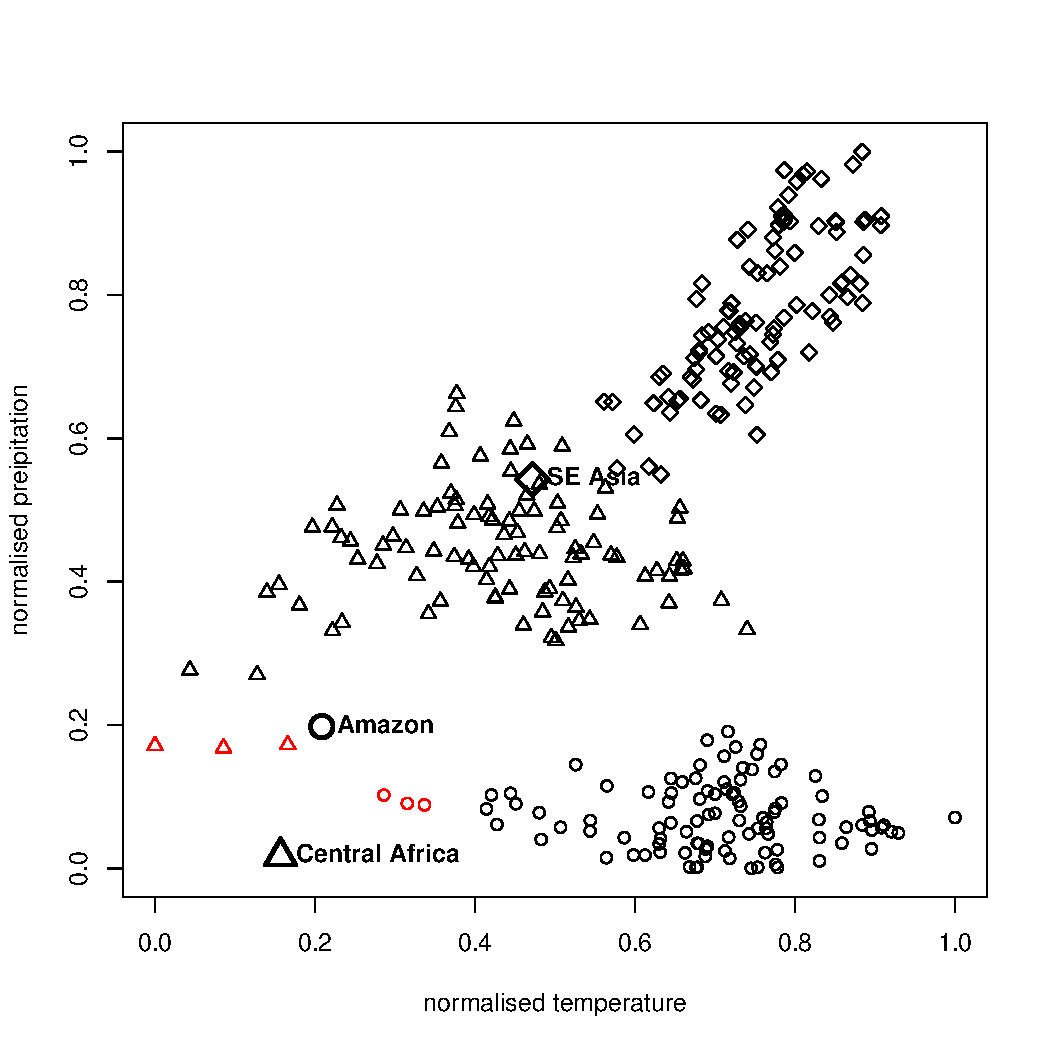
\includegraphics[width=12cm]{../graphics/holdout1_location.pdf}
\caption{Location of held-out ensemble members in temperature and precipitation space.}
\label{fig:holdout1_location}
\end{figure}


Figure \ref{fig:holdout1_vs_loo} shows the prediction of the 6 held-out ensemble members (red dots) in the context of the leave-one-out validation (black dots). In the held-out case, we fit the emulator based on the 294 remaining ensemble members, and predict all 6 held out members at the same time. As the training set is slightly smaller than each leave-one-out training set (299 members), and the emulator is expected to extrapolate further, we might expect a significant degradation in the performance of the emulator in prediction. As we see in fig. \ref{fig:holdout1_vs_loo}, there is little evidence of such a degradation. Both prediction error and estimated uncertainty are well within the bounds of that found during the leave-one-out validation exercise.

\begin{figure}[t]
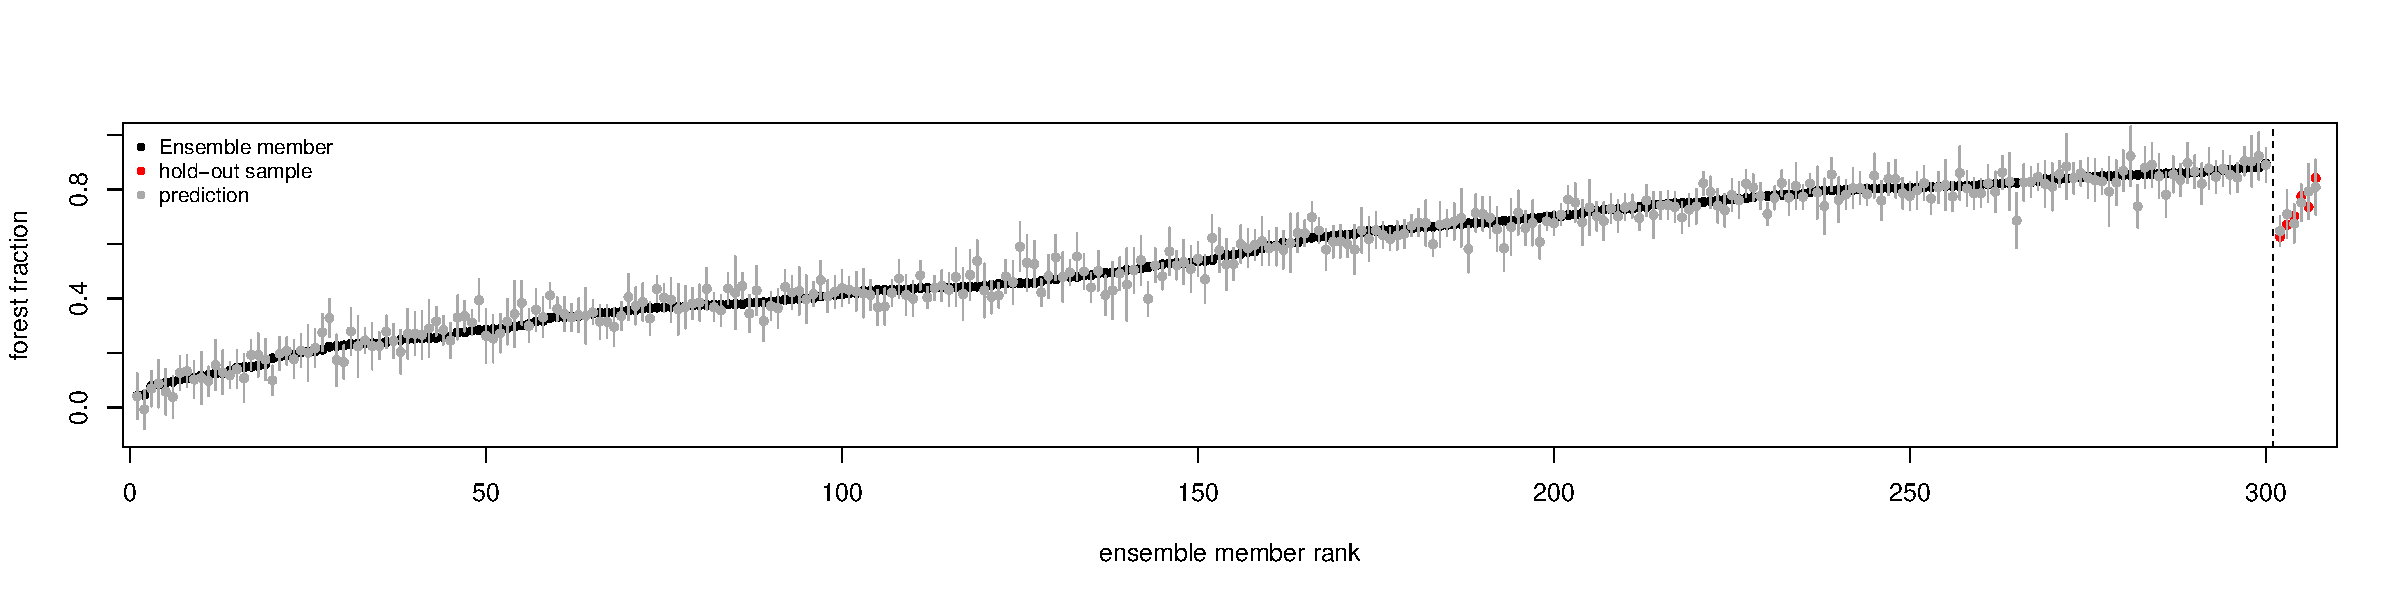
\includegraphics[width=15cm]{../graphics/holdout1_vs_loo.pdf}
\caption{Predictions (grey dots) of forest fraction ensemble members in a leave-one-out validation exercise (black dots) and for the 6 held-out ensemble members (red dots).}
\label{fig:holdout1_vs_loo}
\end{figure}

Figure \ref{fig:holdout1_error_hist} shows the prediction error for the 6 members, in the context of the histogram of errors from the leave-one-out exercise. None of the errors are near the limits of the distribution, even though they might be expected to be larger, with a smaller training set and deeper extrapolation.

\begin{figure}[t]
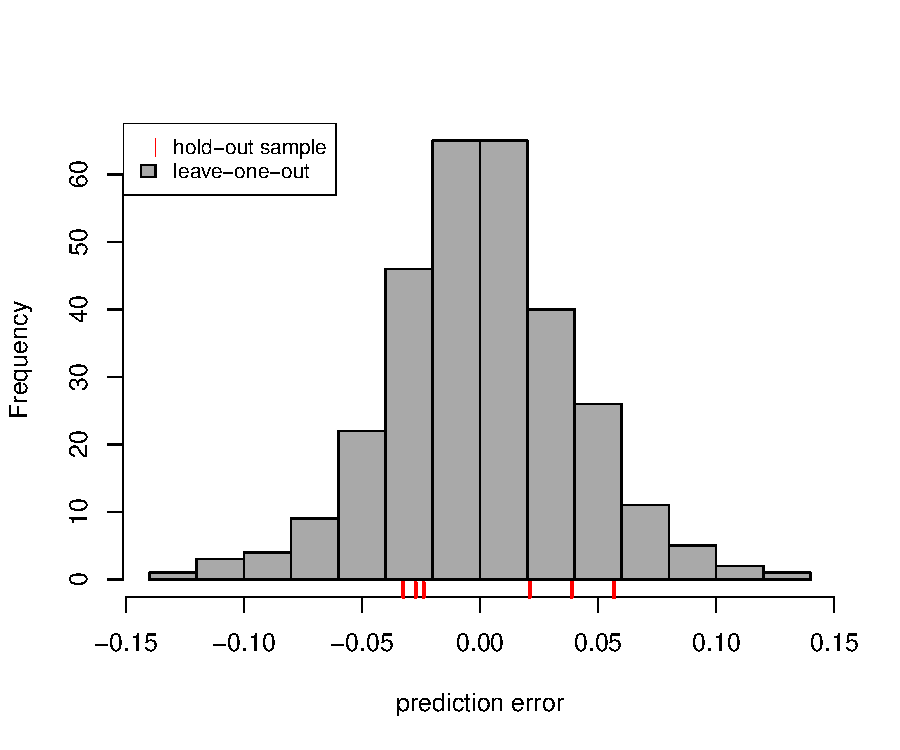
\includegraphics[width=12cm]{../graphics/holdout1_error_hist.pdf}
\caption{Emulator prediction error in the leave-one out validation exercise (grey histogram), with 6 held-out ensemble members.}
\label{fig:holdout1_error_hist}
\end{figure}


When making a direct comparison of prediction of the 6 held-out members (fig. \ref{fig:loo_v_holdout1_prediction_error}), we see that there is some small degradation in the performance of the emulator - predictions tend to be slightly further from the held-out ensemble member, and uncertainty bounds wider. However, it should be noted that the error of the held-out samples is 1) only slightly larger than in the leave-one-out case, 2) small when compared to the range of the ensemble, and 3) prediction uncertainty intervals are certainly appropriate and do not increase dramatically. There seems to be no question that even when asked to predict ensemble members that are near the edge of parameter space, and are a significant extrapolation, the emulator performs well. Obviously, this shouldn’t be taken as meaning that there is no risk of the emulator performing poorly when extrapolating to the regions of the Amazon and Central African temperature and precipitation. However, we hope we have shown that there is little evidence to suggest that the emulator will perform poorly there. 

\begin{figure}[t]
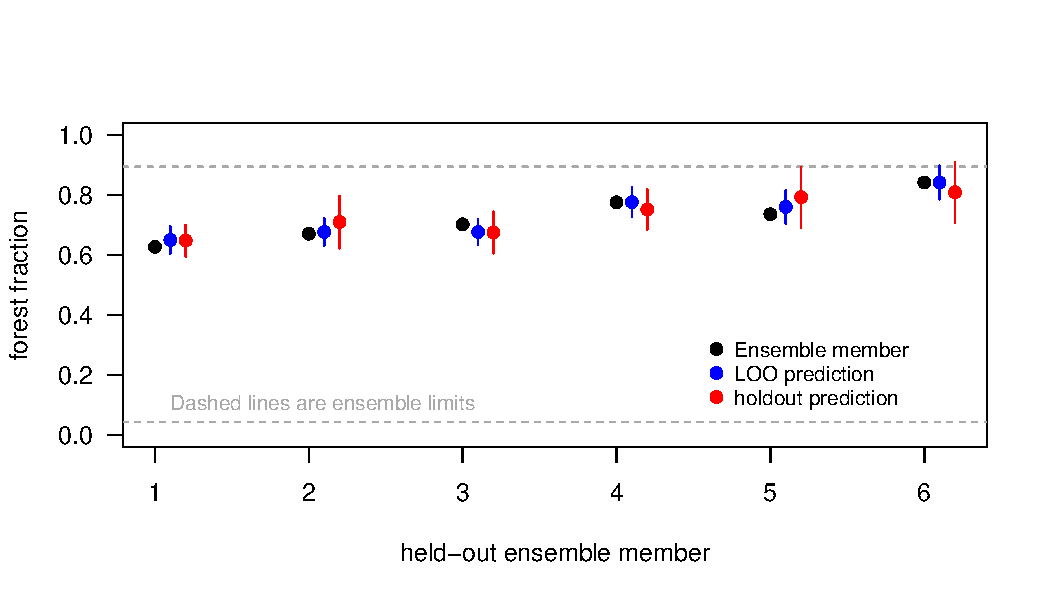
\includegraphics[width=12cm]{../graphics/loo_v_holdout1_prediction_error.pdf}
\caption{Direct comparison of prediction of the held-out ensemble members in both the leave-one-out (LOO, blue points) and held-out (red points) validation exercises.}
\label{fig:loo_v_holdout1_prediction_error}
\end{figure}


\subsection{The importance of the linear prior form for emulator predictions}
We test the importance of the prior form of the emulator may be important in extrapolation to the regions of the observations. In figure \ref{fig:loo_v_holdout_flat_prediction_error}, we look at the error of prediction for an emulator trained using a constant, or “flat” prior form (our standard emulator is built using a linear model prior). We find that the performance of the emulator is very similar in both situations, suggesting that the prior form is not critical in determining the performance of the emulator in extrapolating at least as far as the observations that we have.


\begin{figure}[t]
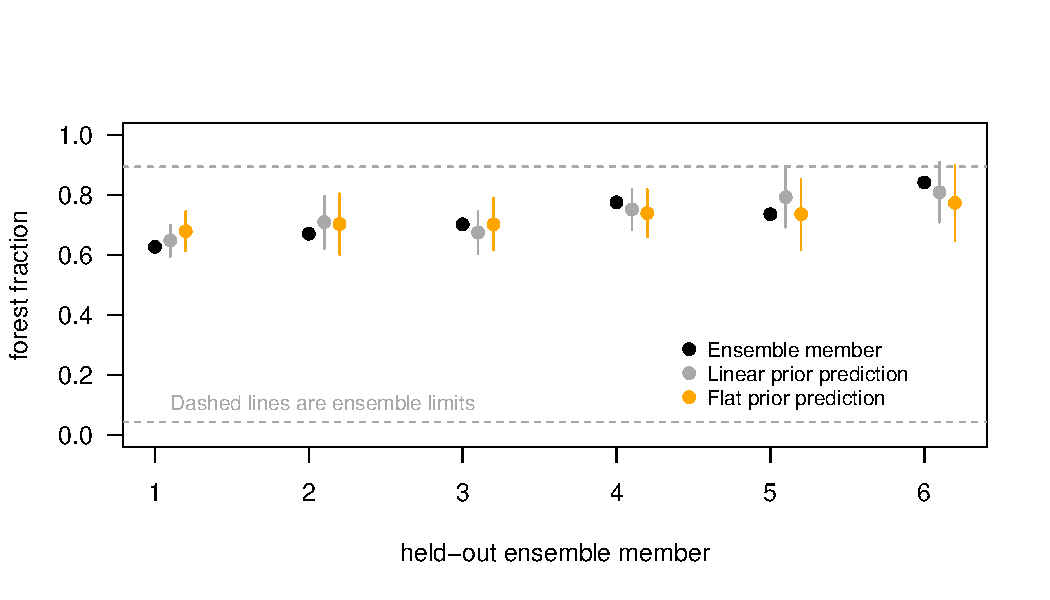
\includegraphics[width=12cm]{../graphics/loo_v_holdout_flat_prediction_error.pdf}
\caption{Comparison of emulators for prediction of held-out ensemble members. Black points are the held-out ensemble members, with grey points representing the standard (linear model prior) emulator, and vertical lines $\pm$ 2 standard deviations. Orange points represent prediction with a ``constant'' or ``flat'' prior, from which the Gaussian process models deviates.}
\label{fig:loo_v_holdout_flat_prediction_error}
\end{figure}



\section{Forest regions}

Forest fraction data is taken by calculating the mean broadleaf forest fraction in the areas shown in figure \ref{fig:map_forests}. Mean temperature and precipitation from the model are calculated for the corresponding regions and time period. The regions are: Amazon 15\textdegree S - 15\textdegree N, 270\textdegree E - 315\textdegree E; Central Africa; 15\textdegree S - 10\textdegree N, 7.5\textdegree E - 30\textdegree E; SE Asia 12\textdegree S - 10\textdegree N, 90\textdegree E - 150\textdegree E.

\begin{figure}[t]
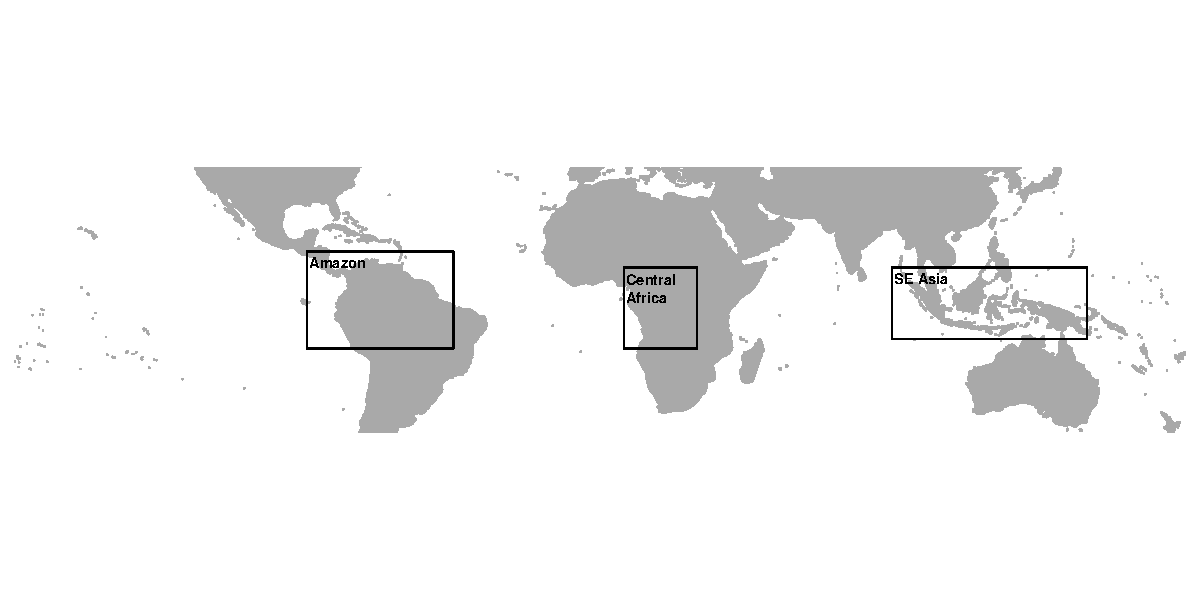
\includegraphics[width=12cm]{../graphics/map_forests_augmented.pdf}
\caption{A map of the forest regions used in the study. }
\label{fig:map_forests}
\end{figure}



\bibliographystyle{copernicus}
\bibliography{augmented.bib}







\end{document}